\section{模式判断需要怎样的联合预言}\label{sec:3-8}

在低能核结构高自旋谱学研究中，研究者常常依据个别能级比值接近某种理想转子或振子规律，或依据观测到一条相对增强的带间跃迁，便赋予实验能带特定的模式标签（如“手征双重带”、“横向摆动带”或“八极反射不对称带”）。然而，正如第\ref{chap:2}章第\ref{sec:2-8}节的综合比较所指出的，不同物理模型由于包含若干可调参数，在低激发能区往往表现出显著的拟合简并。若仅凭能谱局域拟合便断言某种运动模式已确立，容易将参数自由度带来的数值符合误认为物理机制的确证。

为了克服这一局限，本节旨在探讨如何将模式候选转化为具有明确前向预言、最强替代解释和判决性检验路径的研究问题：首先梳理理论模型的前向预言架构与参数输入；进而分析竞争解释在低能区的参数重叠与不可通约性，明确为何不能设立通用的唯象绝对阈值；接着建立包含误差协方差的数据分层架构与留出检验准则；最后基于已有文献原件基线，提出三个具体可证伪的实证研究候选方案（$^{98}\mathrm{Mo}$ 弱跨带电八极跃迁候选、$^{102}\mathrm{Ru}$ 低能偶极响应聚集与 $A \approx 130$ 低自旋取向进动），为后续全书跨质量区实测分析与实验统计反演提供方法论参照。\cite{lawrie-2020-tilted-precession-wobbling,frauendorf-2014-transverse-wobbling,nomura-2022-questioning-wobbling-ibfm,lv-2022-evidence-against-wobbling-135pr,matta-2015-transverse-wobbling-135pr,karmakar-2026-98mo-octupole,saracino-2026-102ru-scissors-octupole-resonances}

\subsection{模式的前向预言结构与模型空间划分}\label{sec:3-8-1}

一个自洽的核结构物理模型，不是事后对实验能级的唯象拟合公式，而是基于明确物理假定对多维物理量的前向映射系统。无论采用全微观自洽理论还是具有明确假定的唯象有效模型，建立一个模式的前向理论预言，均须明确以下四个核心要素：
\begin{enumerate}
\item \textbf{选定的动力学自由度划分}：明确模型保留的主导动力学变量（如转动欧拉角取向坐标、玻尔四极形状坐标 $\beta, \gamma$ 或特定单粒子轨道准粒子算符），以及被冻结或消去的自由度（如高能虚激发或高阶多极形变）。
\item \textbf{守恒量子数与对称性约束}：明确态波函数具有的确定总角动量与宇称 $I^\pi$，以及所保持的离散对称性（如绕内禀主轴旋转 $\pi$ 的签名量子数）。需要特别强调：时间反演 $\hat{\mathcal{T}}$ 是反幺正算符（包含复共轭变换 $i \to -i$），它并不具备普通的线性幺正本征值（不能赋予简单的标量 $\pm 1$ 标签），其动力学约束体现为半整数费米子系统的克喇末简并（$\hat{\mathcal{T}}^2 = -1$）、哈密顿量的时间反演不变性以及电磁跃迁基矢间的确定相位关联。
\item \textbf{势能面与动力学输入}：明确底层势能曲面、转动惯量张量 $\mathcal{J}_k(\omega)$、微观对能隙 $\Delta$ 以及有效跃迁算符。需要指出，具有明确物理自由度与守恒律的唯象有效模型（如固定形变参数的三轴粒子-转子模型 PRM 或代数玻尔哈密顿量），即使未直接耦合全微观自洽的势能曲面（PES），同样能够对能级自旋演化序列与多极电磁跃迁强度给出具有可证伪性的前向预言；而微观能量密度泛函（EDF）与自洽推转计算则进一步为这些唯象参数提供了底层微观机制的支撑。
\item \textbf{拟合参数与前向预言的严格划分}：必须清晰标明哪些实验量被用于固定模型的自由参数（如基态带转动常数或单粒子能隙），独立检验应明确使用未参与拟合的物理量，并核对其与定参数据的共同输入。
\end{enumerate}

需要指出，模型输出的内禀波函数成分分布或半经典相空间角动量进动轨迹（如倾斜进动平面或相空间分离线），仅是特定模型表象下的中间数学表达，其本身并不是直接可观测的实验物理量。将模型标签与实验观测画等号，在认识论上混淆了理论表象与客观物理测量。

\subsection{竞争解释的重叠与固定阈值的局限}\label{sec:3-8-2}

在低自旋区间，不同的微观激发机制常常展现出高度重叠的实验信号特征：
\begin{itemize}
\item 组态相近的准粒子顺排带、具有相同宇称的签名伴带、大振幅 $\gamma$ 软表面激发、三轴倾斜轴进动以及转子摆动运动，在低自旋区间均可能给出近乎相同的能级转动序列，甚至同样伴随带间跃迁。
\item 在传统唯象分析中，常有人试图设定通用的绝对判定阈值（例如硬性规定多极混合比必须满足 $|\delta| > 1$、或带间 $E2$ 分支大于 $50\%$、或二声子激发能必须严格落在单声子能量的两倍附近）。这种通用绝对阈值缺乏微观物理依据：不同核素的单核子壳层占据、三轴形变势阱刚度以及科里奥利退耦点截然不同，不能用单一唯象固定百分比普适认证某种集体运动模式。
\item 在固定门跃迁混合、核取向与几何响应，只将目标跃迁混合比视为未知量的方向角关联（DCO）分析中，比值 $R_{\mathrm{DCO}}(\delta) = W(\theta_1, \theta_2, \phi; \delta) / W(\theta_2, \theta_1, \phi; \delta)$ 表现为两个关于多极混合比 $\delta$ 的二次多项式之比：
\begin{equation}\label{eq:3-8-dco-ratio-form}
R_{\mathrm{DCO}}(\delta) = \frac{a_2 \delta^2 + a_1 \delta + a_0}{b_2 \delta^2 + b_1 \delta + b_0} .
\end{equation}
将式\eqref{eq:3-8-dco-ratio-form}与实验测量值 $R_{\mathrm{exp}}$ 对齐，在排除分母零点以及方程退化情况（即二次项系数非零 $a_2 - R_{\mathrm{exp}} b_2 \neq 0$）后，化简为一个标准一元二次代数方程：
\begin{equation}\label{eq:3-8-dco-quadratic-root}
(a_2 - R_{\mathrm{exp}} b_2)\delta^2 + (a_1 - R_{\mathrm{exp}} b_1)\delta + (a_0 - R_{\mathrm{exp}} b_0) = 0 .
\end{equation}
当判别式大于零时，数学上给出两个实数解。必须明确：
(1) 代数方程的两个根并不天然保证“一大一小”，亦不具备先验的等权概率；
(2) 测量康普顿线偏振度 $P$ 或激发态平均寿命 $\tau$ 在有限实验误差包络内并不能保证在所有情形下排他性排除另一解；
(3) 因此，谱学反演应完整报告相容的根分支及其非对称误差包络，避免依据特定模型偏好主观剔除物理实根。
\item 此外，光子多极混合比 $\delta(E2/M1)$ 严格由第\ref{sec:5-9}节给出的出射辐射场发射几率振幅之比定义，包含了跃迁辐射能量因子、波长与明确的电磁耦合算符约定。若磁辐射算符采用国际单位制（SI）电荷型约定 $\mathcal{M}_S(M1) \equiv \mathcal{M}_\mu(M1)/c$（具有电荷乘长度量纲 $e\cdot\mathrm{fm}$），波数因子 $E_\gamma/(\hbar c)$（量纲 $\mathrm{fm}^{-1}$）与电四极算符 $\mathcal{M}(E2)$（量纲 $e\cdot\mathrm{fm}^2$）相配，保证 $\delta$ 成为严格无量纲振幅比：
\begin{equation}\label{eq:3-8-delta-def}
\delta(E2/M1) = \frac{\sqrt{3}}{10} \frac{E_\gamma}{\hbar c} \frac{\langle I_f \| \hat{\mathcal{M}}(E2) \| I_i \rangle}{\langle I_f \| \hat{\mathcal{M}}_S(M1) \| I_i \rangle} = \frac{\sqrt{3}}{10} \frac{E_\gamma}{\hbar} \frac{\langle I_f \| \hat{\mathcal{M}}(E2) \| I_i \rangle}{\langle I_f \| \hat{\mathcal{M}}_\mu(M1) \| I_i \rangle} .
\end{equation}
本式沿用第\ref{sec:5-9}节配套的发射振幅、算符相位与几何系数约定；单独指定 SI 单位并不足以决定混合比符号。式\eqref{eq:3-8-delta-def}表明，$\delta$ 绝不是裸的电四极与磁偶极约化矩阵元比值（RME Ratio）。当分母上的磁偶极矩阵元因几何进动取向或单粒子自旋选择定则受到强烈压低时，即使带间电四极跃迁强度未发生任何集体增强，数值上仍可导出可观的 $|\delta|$；反之，若分母 $M1$ 强度很大，较小的 $|\delta|$ 亦不必然否定集体 $E2$ 成分的存在。绝对折合跃迁几率 $B(E2)$ 与相对混合比 $\delta$ 提供互补的绝对标度与干涉信息，在谱学分析中往往通过寿命、角关联与偏振的联合拟合共同约束，不可假设二者在统计上完全独立。
\end{itemize}

\subsection{独立观测量的协方差与四层数据架构}\label{sec:3-8-3}

在评估实验证据对理论模型的支持度时，必须审慎考察观测量之间的统计关联与归一规范：
\begin{enumerate}
\item \textbf{跃迁速率、寿命与分支比的精确关系}：设某一激发母态的平均寿命为 $\tau$（对应总衰变几率 $\lambda_{\mathrm{tot}} = 1/\tau = \sum_j \lambda_{\mathrm{tot}, j}$）。对于由该母态发出的第 $i$ 条退激分支：
\begin{itemize}
\item 若已知包含光子衰变与内转换电子（IC）的总分支比 $b_{\mathrm{tot}, i} \equiv \Gamma_i / \Gamma_{\mathrm{tot}}$，则部分光子跃迁速率为：
\begin{equation}\label{eq:3-8-b-rate-relation}
\lambda_{\gamma, i} = \frac{b_{\mathrm{tot}, i}}{\tau (1 + \alpha_{\mathrm{tot}, i})} ,
\end{equation}
其中 $\alpha_{\mathrm{tot}, i}$ 为该跃迁的总内转换系数。
\item 若实验直接定义并给出纯光子发射概率（光子分支比）$b_{\gamma, i} \equiv \Gamma_{\gamma, i} / \Gamma_{\mathrm{tot}}$，则光子跃迁速率直接由定义给出：
\begin{equation}\label{eq:3-8-b-rate-direct}
\lambda_{\gamma, i} = \frac{b_{\gamma, i}}{\tau} ,
\end{equation}
此时分母绝不可再次额外除以 $(1 + \alpha_{\mathrm{tot}, i})$，否则将引入内转换因子的虚假重复扣除。
\item 若实验仅测得由同一母态退激的各光子相对强度 $I_{\gamma, j}$，则该分支的部分光子跃迁速率必须通过母态所有退激出口的完整求和归一给出：
\begin{equation}\label{eq:3-8-lambda-relative}
\lambda_{\gamma, i} = \frac{I_{\gamma, i}}{\tau \left[ \sum_j I_{\gamma, j} (1 + \alpha_{\mathrm{tot}, j}) + I_{\mathrm{other}} \right]} ,
\end{equation}
其中 $I_{\mathrm{other}}$ 必须是与所列强度采用相同任意归一刻度的其他出口权重；未知出口不能仅靠给它命名便视为已知，其影响应保留为缺失分支界限或拟合参数。
\end{itemize}
在固定跃迁能量与分支比时，实验提取的折合跃迁几率满足 $B(\sigma L) \propto \lambda_\gamma / E_\gamma^{2L+1}$，严格反比于母态平均寿命 $\tau$（$B \propto 1/\tau$），随寿命变短而增大，决非随寿命增加而增大。
\item \textbf{四类协方差机制的严格区分}：从同一激发母态退激的多个跃迁分支共享母态寿命 $\tau$ 与共用的全探测阵列效率刻度，使得派生出的多个跃迁绝对几率 $B(\sigma L)$ 之间存在统计关联。在核谱学数据处理中，必须细致区分四类性质不同的协方差机制：
\begin{itemize}
\item \textbf{刻度协方差 (Calibration Covariance)}：来自全能峰效率曲线的全局拟合不确定度、靶厚与束流积分归一化因子，使同一实验测得的所有绝对强度产生联动；
\item \textbf{拟合参数协方差 (Fitting Covariance)}：能谱重叠峰非线性拟合中峰位、半高宽与峰面积之间的协方差；
\item \textbf{留出检验协方差 (Holdout Covariance)}：在多维参数空间中，若检验集与训练集共享中间标定参数，将削弱留出检验的条件独立性；
\item \textbf{同采集协方差 (Co-acquisition Covariance)}：同一次核反应中由于相同复合核布居历史、复杂的侧馈送（side-feeding）时间延迟及同一母态寿命所引起的物理量统计关联。需要说明，这些协方差机制在实际数据中相互交织，共享物理因素并不必然导致所有参数间的相关系数都呈现强正相关。
\end{itemize}
\item \textbf{能谱调参不属于留出验证}：利用同一核素的低自旋能级拟合模型参数后，再次用该模型计算同一能谱的吻合程度，仅属于自洽闭环拟合，不具备独立的检验效力。自洽的模型验证必须将已调参数严格固定，并在完全未参与参数调整的“留出观测空间”中接受检验。
\item \textbf{四层数据架构}：为了避免证据层级的混淆，研究中必须严格区分四类数据载荷：
\begin{itemize}
\item \textbf{原始测量量 (Raw Data)}：探测器原始脉冲计数、符合矩阵、原始各向异性角分布计数；
\item \textbf{采用物理量 (Adopted Properties)}：经探测器响应反演后的能级能量、激发态半衰期 $T_{1/2}$；
\item \textbf{派生跃迁量 (Derived Observables)}：结合分支比与转换系数计算出的绝对折合跃迁几率 $B(E2), B(M1)$ 及拟合提取的混合比 $\delta$；
\item \textbf{理论模型输出 (Model Quantities)}：模型本征能量、组态混合矩阵元与相空间角动量轨迹。
\end{itemize}
\end{enumerate}

在进行模型预言与实验数据的定量比对时，残差向量定义为 $\mathbf{r} = \mathbf{y}_{\mathrm{exp}} - \mathbf{y}_{\mathrm{model}}$。在明确的矩条件或渐近高斯假定下，已知实验报告的测量中心值向量 $\mathbf{y}_{\mathrm{exp}}$ 与完整协方差矩阵 $\mathbf{V}$，可通过广义最小二乘加权距离 $\chi^2 = \mathbf{r}^T \mathbf{V}^{-1} \mathbf{r}$ 进行条件拟合推断。需要指出：若各个分支比在分析中被强行归一化（$\sum_j b_j = 1$），则全协方差矩阵 $\mathbf{V}$ 存在代数约束因而数学上必定是奇异矩阵（行列式为零），此时必须选取独立的无约束坐标子集或采用约束广义逆度规进行自洽求解。

\subsection{三个可证伪的实证研究候选}\label{sec:3-8-4}

基于上述方法论标准，本小节提出三个具有确凿文献原件基线、物理机制明确且具备可操作判决路径的实证研究候选方案。

\paragraph{候选一：$^{98}\mathrm{Mo}$ 弱跨带电八极跃迁候选与八极动力学检验}
在 $A \approx 100$ 质量区的过渡区偶偶核 $^{98}\mathrm{Mo}$（$Z=42, N=56$）中，Karmakar 等人在近期高自旋谱学实验中报道了连接负宇称带与正宇称带的两条弱跨带跃迁候选。\cite{karmakar-2026-98mo-octupole}
\begin{itemize}
\item \textbf{已有测量事实与多极界限}：Karmakar 等人利用加尔各答变能量回旋加速器中心（VECC）的 11 台 Clover 探测器阵列，通过 $45\,\mathrm{MeV}\ ^4\mathrm{He}$ 束流轰击 $^{100}\mathrm{Mo}$ 靶开展 $^{100}\mathrm{Mo}(\alpha, \alpha 2n)^{98}\mathrm{Mo}$ 反应，测定了 $^{98}\mathrm{Mo}$ 的高自旋能级结构。在原文表 1（文献第 4 页）报告的 31 条伽马跃迁中，全谱相对强度以最强的基态带 $787.2(3)\,\mathrm{keV}\ 2_1^+ \to 0_1^+$ 跃迁为基准定为 $100.0(30)$。实验确立了两个关键负宇称母态的退激路径：
对于 $2620.4(3)\,\mathrm{keV}\ 5^-$ 母态，退激分支包含带内四极跃迁 $603.1(2)\,\mathrm{keV}\ 5^- \to 3^-$（$I_\gamma = 8.94(45)$，实验指认为 $E2$）、偶极跨带跃迁 $1110.8(3)\,\mathrm{keV}\ 5^- \to 4_1^+$（$I_\gamma = 10.33(55)$，实验指认为 $E1$）以及微弱的跨带跃迁 $1833.3(5)\,\mathrm{keV}\ 5^- \to 2_1^+$（$I_\gamma = 0.24(9)$）；
对于 $3095.4(4)\,\mathrm{keV}\ 7^-$ 母态，退激分支包含带内四极跃迁 $475.1(2)\,\mathrm{keV}\ 7^- \to 5^-$（$I_\gamma = 9.89(25)$，实验指认为 $E2$）、偶极跨带跃迁 $752.4(3)\,\mathrm{keV}\ 7^- \to 6_1^+$（$I_\gamma = 8.52(40)$，实验指认为 $E1$）以及微弱的跨带跃迁 $1585.8(6)\,\mathrm{keV}\ 7^- \to 4_1^+$（$I_\gamma = 0.74(16)$）。
必须强调：表 1 中这两条弱跃迁的角关联比值 $R_{\mathrm{DCO}}$ 与偏振不对称度 $\Delta_{\mathrm{iPDCO}}$ 栏均为空白（未测定），由初末态自旋宇称差确定电八极 $E3$ 仅为其角动量允许的最低阶次，实验并未排他性排除更高阶多极混合。全谱相对强度 $I_\gamma = 0.24(9)$ 与 $0.74(16)$ 不能直接等同于母态自身的分支比，将其转换为部分衰变率必须考虑同一母态其它退激通道的条件归一、内转换系数及未观测支路的边界。
\item \textbf{尚缺关键数据与强替代解释}：目前负宇称母态 $5^-$ 与 $7^-$ 的激发态绝对寿命 $\tau$ 均未测得。原作者在纯 $E3$ 多极假定下，在原文表 2（文献第 6 页）报告了相对强度比值与折合跃迁几率比值：对于 $5^-$ 态，强度比 $I_\gamma(E3)/I_\gamma(E2) = [I_\gamma(1833.3)/I_\gamma(603.1)] = (2.68 \pm 1.01) \times 10^{-2}$，推导出 $B(E3)/B(E2) = 66.05 \pm 27.01\,\mathrm{fm}^2$；对于 $7^-$ 态，强度比 $I_\gamma(E3)/I_\gamma(E2) = [I_\gamma(1585.8)/I_\gamma(475.1)] = (7.48 \pm 1.62) \times 10^{-2}$，推导出 $B(E3)/B(E2) = 153.81 \pm 33.31\,\mathrm{fm}^2$。这一比值存在两种相互竞争的微观解释：(1) 负宇称带具有显著的内禀八极集体关联，八极矩阵元 $\langle 2_1^+ \| \mathcal{M}(E3) \| 5^- \rangle$ 发生集体增强；(2) 作为比值分母的带内四极跃迁 $B(E2; 5^- \to 3^-)$ 因初末态单粒子组态重构或核形状突变而受到严重结构阻碍。在缺乏绝对寿命的情况下，无法判定大比值究竟来自分子八极增强还是分母四极受阻。
\item \textbf{可执行的实验判决与可证伪条件}：检验上述八极集体假说，核心在于测定母态 $5^-$ 与 $7^-$ 的绝对寿命 $\tau$。一条可检验的实验路线是：不必仅在在统计微弱的跨带跃迁（$I_\gamma = 0.24$）上线形反演，而是可以通过高重符合门技术，在较强的同母态退激跃迁（如 $5^-$ 态的 $603.1\,\mathrm{keV}$ 或 $1110.8\,\mathrm{keV}$，以及 $7^-$ 态的 $475.1\,\mathrm{keV}$ 或 $752.4\,\mathrm{keV}$）上线形反演或反冲距离法提取母态寿命。方法选择须基于具体核动力学约束：预期多普勒频移展宽 $\Delta E_\gamma = E_\gamma (v/c) \cos\theta$ 与探测器能量分辨的比值决定了多普勒频移衰减法（DSAM）的灵敏窗口，可用寿命窗口还取决于反冲核在靶与衬底中的慢化剖面、响应展宽和侧馈入，不宜预设统一的皮秒阈值；而微米级反冲距离法（RDM/Plunger）则要求反冲飞行距离 $v\tau$ 与机械间距精度相匹配。若精确测得的绝对寿命结合分支比表明，带内四极跃迁 $B(E2)$ 显著受到阻碍，而绝对八极跃迁几率 $B(E3)$ 仅处于单核子 Weisskopf 估算区间，则会排除预言该支路显著增强的具体模型实现；反之，若绝对 $B(E3)$ 与其同母态网络符合集体计算，则会增加该核存在八极关联的证据，但仍需区分动态关联与稳定形变。
\end{itemize}

\paragraph{候选二：$^{102}\mathrm{Ru}$ 低能偶极响应聚集与八极共振结构检验}
在过渡区核素 $^{102}\mathrm{Ru}$（$Z=44, N=58$）中，Saracino 等人利用 TUNL-HIGS 的线偏振准单能光子束开展了高灵敏核共振荧光（NRF）测量，研究了低激发区的偶极跃迁强度分布。\cite{saracino-2026-102ru-scissors-octupole-resonances}
\begin{itemize}
\item \textbf{已有测量事实与截面约束}：NRF 实验测量的直接物理观测量是散射截面角分布积分 $I_s \propto g \Gamma_0^2 / \Gamma$（其中 $\Gamma_0$ 为跃迁回基态的部分宽度，$\Gamma$ 为全衰变宽度），直接约束的是 $\Gamma_0^2/\Gamma$，全跃迁强度的精确提取依赖于基态分支比 $\Gamma_0/\Gamma$。实验在 $2\sim 4\,\mathrm{MeV}$ 能区测定了磁偶极剪刀模响应（$\sum B(M1)\!\uparrow \approx 1.0\,\mu_N^2$）；并在电偶极通道确立了特征信号：在 $2.95\,\mathrm{MeV}$ 处测得一条孤立的强 $E1$ 跃迁（原文图 2 注列出能量为 $2953.2(19)\,\mathrm{keV}$），提取出 $B(E1)\!\uparrow = 0.016\,e^2\mathrm{fm}^2$；同时在 $4.5\sim 5.5\,\mathrm{MeV}$ 能区（中心在 $4.9\,\mathrm{MeV}$ 附近）观测到显著的 $E1$ 强度聚集，累积积分强度约为 $\sum B(E1)\!\uparrow \approx 0.1\,e^2\mathrm{fm}^2$。
\item \textbf{多极选择定则与有效算符边界}：偶偶核基态为 $0^+$，直接单光子吸收激发的 $1^-$ 态严格遵循电偶极选择定则（$|0 - 1| \le \lambda \le 0 + 1 \implies \lambda = 1, \Delta\pi = -$），因此从基态直接进行的 NRF 吸收测量是纯粹的 $E1$ 跃迁，绝非对该状态直接进行电八极 $E3$ 激发（直接 $E3$ 激发只能布居到 $3^-$ 态）。Saracino 等人采用的 TAC-QRPA 理论模型中引入的诱导八极极化项 $O(E1;\nu) = e_{\mathrm{eff}} r Y_{1\nu} + e_{\mathrm{eff}} b_\nu r^3 Y_{3\nu}$ 属于内禀坐标系下的唯象分量表达，非实验室系下严格的 1 阶不可约球张量；在旋转协变的有效算符展开中，可以包含四极与八极张量耦合成秩1的项（$T_M^{(1)} = D_M^{(1)} + c \sum_{m,k} C_{2m 3k}^{1M} Q_{2m} O_{3k}$），该项的系数及截断仍依赖具体模型；八极算符本身是秩3张量，不能直接当作实验室秩1的单光子吸收算符。
\item \textbf{二声子假说与多通道判决路径}：Saracino 等人在文献第 6 页推测 $2.95\,\mathrm{MeV}$ 孤立态可能属于四极-八极二声子构型 $[2_1^+ \otimes 3_1^-]_{1^-}$，文献指出该构型的激发能量预期在单声子能量之和 $E(2_1^+) + E(3_1^-) = 2518\,\mathrm{keV}$ 附近。在理想谐振子微观图像下，二声子态向单声子八极态 $3_1^-$ 的退激具备集体四极跃迁特征，预言其折合跃迁几率 $B(E2; [2_1^+ \otimes 3_1^-]_{1^-} \to 3_1^-) \approx B(E2; 2_1^+ \to 0_1^+)$。必须清醒认识到：跃迁速率与光子分支比不仅取决于折合几率 $B(\sigma L)$，更强烈依赖于跃迁能量的相空间因子（$\lambda \propto E_\gamma^{2L+1} B$）。在 $^{102}\mathrm{Ru}$ 中，退激回基态的 $E1$ 跃迁能量高达约 $2.95\,\mathrm{MeV}$（按 $E_\gamma^3$ 贡献），而向单声子八极态 $3_1^-$ 的带间 $E2$ 跃迁能量仅为两能级之差 $\Delta E = E(1^-) - E(3_1^-)$（按 $E_\gamma^5$ 贡献）。能量因子的幂次差异与辐射常数抑制，导致即使该带间 $E2$ 具备完全集体的 $B(E2)$ 强度，其实际光子分支比仍可能远小于基态强 $E1$ 分支；此外低能跃迁还伴随内转换电子（ICC）分流。因此，不能将“带间四极分支必须主导”作为二声子模式成立的前提。实验检验必须通过高灵敏在束符合伽马谱学或多步库仑激发，综合测定向 $3_1^-$ 的退激分支与全衰变网络并提取绝对跃迁几率：若实测绝对强度证实带间 $B(E2)$ 显著受到非相干准粒子成分的阻碍，则相干四极-八极二声子共振耦合假说在该核区被削弱。
\end{itemize}

\paragraph{候选三：$A \approx 130$ 奇 $A$ 核低自旋取向进动模式的判决路径}
在典型的过渡区奇 $A$ 核（以 $^{135}\mathrm{Pr}$ 与 $^{133}\mathrm{La}$ 为代表）中，围绕基于奇质子 $h_{11/2}$ 轨道的低自旋负宇称能带动力学机制存在长期的学术争论。\cite{lawrie-2020-tilted-precession-wobbling,frauendorf-2014-transverse-wobbling,nomura-2022-questioning-wobbling-ibfm,lv-2022-evidence-against-wobbling-135pr,matta-2015-transverse-wobbling-135pr}
\begin{itemize}
\item \textbf{实验争议与双根多解分支}：在奇质子核 $^{135}\mathrm{Pr}$（$Z=59, N=76$）中，负宇称转动带带头自旋为 $11/2^-$，其伴带连接跃迁涉及 $17/2^-$ 与 $15/2^-$ 等负宇称态。Matta 等人基于早先在束角分布实验中提取的较大多极混合比分支（$|\delta| \approx 2.5$），将伴带解释为横向摆动运动（Transverse Wobbling）的实验证据~\cite{matta-2015-transverse-wobbling-135pr}；然而，Lv 等人开展的独立在束实验利用 Clover 探测器阵列测定了严格的康普顿线偏振度，证实其实验角分布与偏振数据高度相容于以磁偶极为主导的小混合比分支（对关键带间连接跃迁 $747.3\,\mathrm{keV}\ 17/2^- \to 15/2^-$ 提取出 $\delta = -0.47^{+0.09}_{-0.22}$）~\cite{lv-2022-evidence-against-wobbling-135pr}。不同研究团队得出的对立结论，并非由形变坐标的先验偏好所单一决定，而是真实反映了这些实验设置下角分布反演的多解性，以及联合响应、取向与统计处理的差异。
\item \textbf{三类竞争模型及其可证伪判据}：在理论解释上，针对该能带存在三类相互竞争的微观与唯象实现：(1) 冻结短轴顺排粒子-转子模型（Frauendorf-Dönau 2014），以明确的惯量和组态预言带间电磁强度；其与观测相容性需同时检验混合比分支；(2) 准粒子-三轴转子的完整取向解及 TiP 描述，其中 Lv 等人 2022 的 QTR 计算放开准粒子取向，而 Lawrie 等人 2020 以冻结准粒子的对照计算检验摆动近似；两者不能视为同一实现；(3) 相互作用玻色子-费米子模型（IBFM，Nomura 与 Petrache 2022），考察 $\gamma$ 软核芯与奇核子耦合产生的激发序列。判决这三类模型不能依靠通用的唯象绝对阈值，而应为各模型规定可比较的输入约束及参数不确定度，再比较共同可观测量；IBFM 与 PRM 的内部参数不必具有逐个一一对应：利用微米级反冲距离法（RDM）测定 $17/2^-$ 态的绝对寿命，结合完整分支、转换系数、角关联和偏振的相容解，提取带间绝对 $B(E2)$ 与 $B(M1)$；若在相同误差与分支条件下，实测 $B(E2)$ 显著低于 Frauendorf-Dönau 冻结短轴摆动模型在该核区给出的前向预测区间，则该具体横向摆动实现及其输入范围将与这一组数据不相容。
\end{itemize}

\subsection{跨质量区迁移准则与全书判据总结}\label{sec:3-8-5}

图\ref{fig:3-8-joint-workflow}概括了从理论模型空间出发，经由包含统计协方差的多维互补信息通道，最终落地于实证研究候选方案的整体逻辑流程。

\begin{figure}[htbp]
\centering
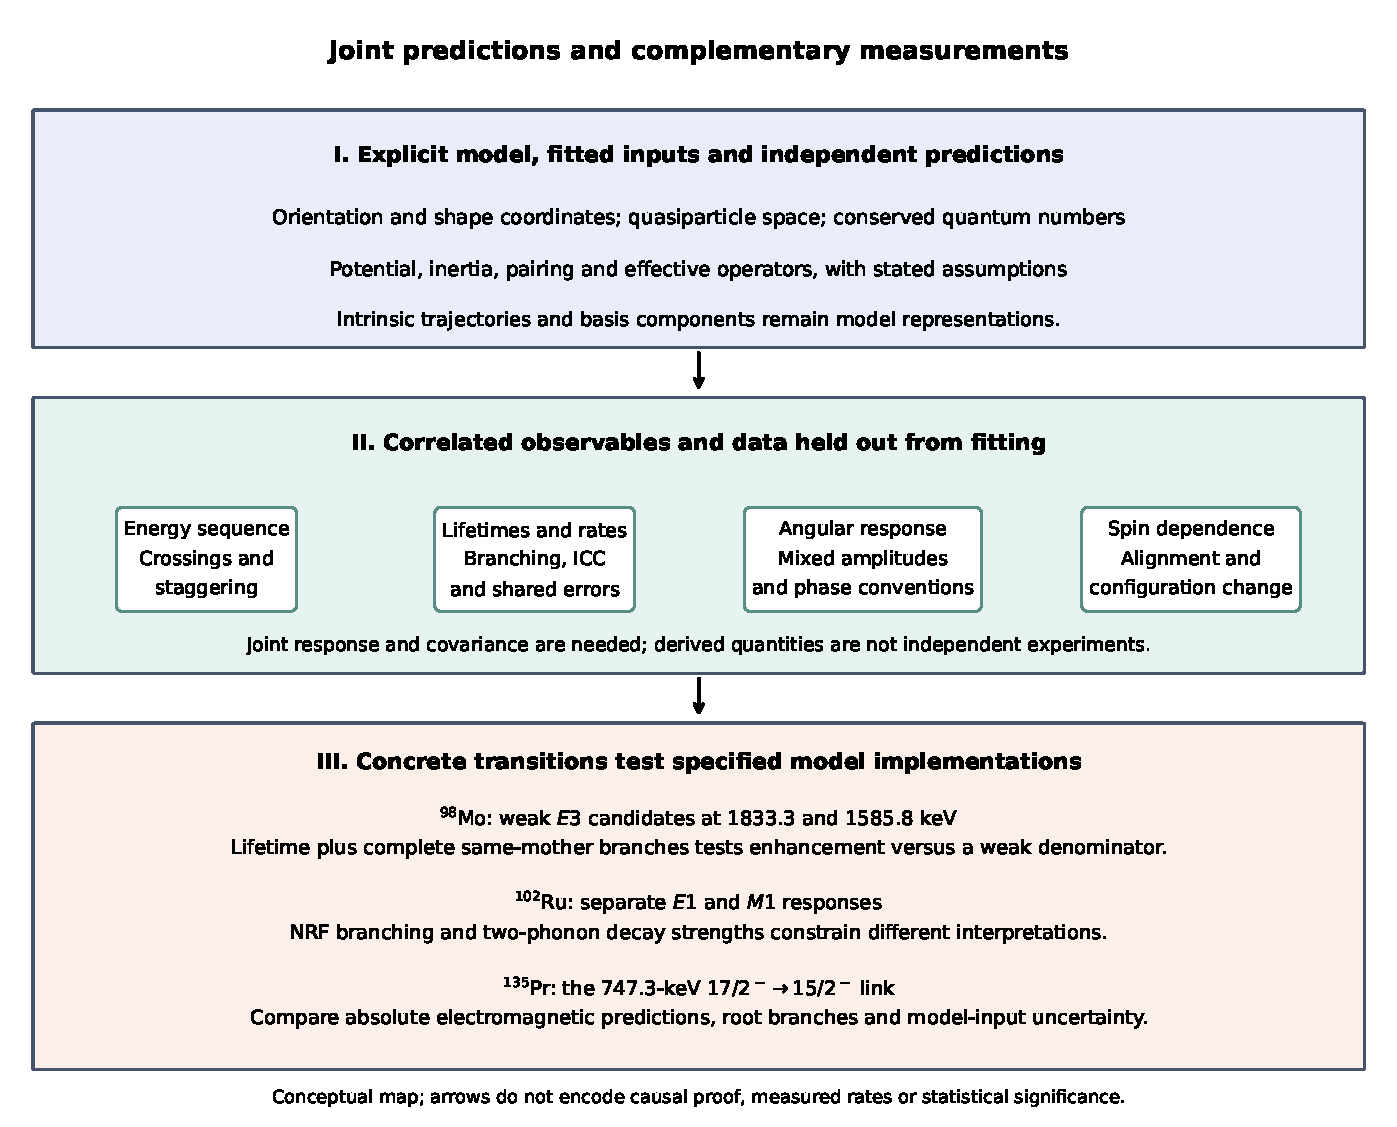
\includegraphics[width=0.88\textwidth]{Img/joint-predictions-workflow.pdf}
\caption[模式判断需要怎样的联合预言：理论前向预言架构、互补信息通道与实证研究候选逻辑框架示意图]{模式判断需要怎样的联合预言：理论前向预言架构、互补信息通道与实证研究候选逻辑框架示意图。图示展示了从理论模型自由度划分与输入设定出发，经由多通道关联实验观测（能级序列、绝对衰变速率、方向角关联双根与偏振度、高自旋顺排响应），最终落地于具体可证伪实证候选的科学闭环；代码实现与数据来源参见附录\ref{app:reproducible-inputs}。}\label{fig:3-8-joint-workflow}
\end{figure}

当将某一特定核区（如 $A \approx 130$ 区）总结出的模式机制推广迁移至其它质量区时，必须严格遵守微观自洽的物理迁移准则：
\begin{itemize}
\item 必须逐一核查目标核区的微观费米面轨道占据情况、自旋-轨道伴对轨道的相对劈裂、质子-中子残余相互作用的有效强度（如Ding 等人在 $A \approx 60$ 钴同位素探索性三轴粒子-转子计算中对残余力 $V_{pn}$ 与取向进动边界的系统考察~\cite{ding-2025-chiral-rotation-a60-residual-interactions}）、自洽平均场势能面的三轴刚度、以及在束反应布居通道的角动量输入特征。
\item 不能仅因某个质量数区间与已知变形核相近，或因文献暂缺，便断言新模式的『确证』或『缺失』。原子核的多体激发动力学由其微观壳层结构与哈密顿量本征态决定，模式判断应以具体实验证据与反例检验为准。
\end{itemize}

综上所述，将一个理论模式确立为真实客观的核物理激发，绝非依赖孤立的能谱拟合或人为的模式命名，而是依赖于一组具有互补信息维度、相互自洽的联合预言链条。通过建立包含绝对寿命、多角度偏振分析、高自旋顺排演化以及严格考量统计协方差的多维观测体系，并面向具体实证候选开展判决性测量，才能真正打破模型解释简并，将低能核结构高自旋谱学研究推进至自洽严谨的科学高度。
